\documentclass[12pt]{article}
\usepackage[latin1]{inputenc}
\usepackage[italian]{babel}
\usepackage{microtype} % tipografia
\usepackage{graphicx}
\usepackage[bookmarks=true,bookmarksopen=true,pdfhighlight=/I,pdfpagemode=UseOutlines]{hyperref} % hyper-links, questo va per ultimo


\makeindex

\begin{document}
\title{Relazione del progetto di \\Sistemi Distribuiti}
\author{Elia Calligaris e Paolo Snidaro}
\date{\textit{bozza} - \today}
\maketitle
\tableofcontents

\section{Introduzione}\label{sec:intro}

Il problema proposto � quello di implementare un protocollo di transazioni distribuite, tramite il quale dei client possono prenotare in modo concorrente delle risorse disposte su pi� server.

\paragraph{Il pretesto} � quello di gestire un sistema di prenotazione di posti su voli aerei. Idealmente un'agenzia di viaggio (client) deve essere in grado di prenotare via internet una serie di posti su pi� voli di diverse compagnie. I server delle compagnie aeree mantengono la lista e lo stato dei voli e relativi posti. La prenotazione ha successo se e solo se \textit{tutti} i posti richiesti vengono prenotati. 

Naturalmente si vuole evitare che le richieste di prenotazione interferiscono tra di loro (e soprattutto evitare che lo stesso posto venga prenotato pi� volte). %Nel caso in cui venga richiesto un posto che risulta occupato, il client potrebbe proporre un posto alternativo all'utente (se possibile).

\paragraph{Una soluzione na\"ive} � quella di creare una transazione per ogni posto da prenotare, abortendo nel caso in cui una fallisca; tuttavia si vuole evitare l'annullamento di prenotazioni gi� effettuate.

%============================================================================
%============================================================================
%============================================================================

\section{Analisi}\label{sec:analisi}

\subsection{Requisiti funzionali}
\begin{itemize}
	\item Ogni agenzia deve poter richiedere i voli e i posti disponibili alle compagnie.
	\item Ogni agenzia deve essere in grado di prenotare atomicamente una serie di posti su voli potenzialmente diversi. A fronte della lista di posti richiesti, viene richiesta la conferma o meno della prenotazione, eventualmente con delle proposte alternative a posti richiesti ma occupati.
	\item Qualora un'agenzia non riesca ad ottenere uno o pi� posti richiesti, l'intera prenotazione deve essere annullata.
	\item Qualora un client (agenzia) subisca guasti, la transazione va abortita.
	\item Ci devono essere almeno cinque compagnie aeree.
	\item Ogni server di ogni compagnia aerea mantiene una lista di voli, i quali hanno una serie di posti che possono essere liberi o prenotati.
	\item Un posto in aereo non deve mai venire prenotato pi� volte.
	\item Una volta confermata una prenotazione per un posto aereo, questa non deve essere pi� annullata dai server.
	\item L'agenzia deve essere in grado di disdire una prenotazione. Si astrae su eventuali termini per l'annullamento.
\end{itemize}

\subsection{Requisiti non funzionali}

\begin{itemize}
	\item Alta disponibilit�, almeno $96\%$ (circa un giorno al mese di downtime).
	\item Tempi di risposta contenuti: se una transazione non viene completata entro $N$ secondi, viene abortita (dal client).
		\item Trasparenza rispetto alla replicazione. Una stessa compagnia pu� avere pi� server replica; pu� esporli tutti su indirizzi separati, oppure metterli sotto un singolo indirizzo e gestirli come pi� opportuno. Se vengono esposti pi� indirizzi, sar� il client a contattarne di diversi in caso di problemi.
\end{itemize}
\subsubsection{Fault Tolerance}
\begin{itemize}
	\item I server delle compagnie aeree devono cercare di mascherare i \textit{crash}. Un crash durante una transazione causa un \textit{abort}, uno dopo il \textit{commit} non deve causare perdite.
	\item Omissioni di messaggi da parte dei server vengono visti dal client come un \textit{timeout}. Se sono disponibili indirizzi alternativi, il client pu� decidere di contattarli in modo trasparente.
	\item Omissioni o crash da parte del client portano la transazione ad essere abortita dai server.
\end{itemize}

%============================================================================
%============================================================================
%============================================================================

\section{Progetto e specifiche}

\subsection{Architettura logica}
% Componenti, funzioni, utenti

L'architettura � di tipo \textit{client-server} a due \textit{tier}, con server \textit{peer} (dato che le risorse sono distribuite).

I \textbf{server} delle compagnie aeree mantengono la lista di voli e di posti a sedere, tendendo conto se quest'ultimi sono occupati o meno (e da chi). Forniscono la lista dei posti su richiesta. Possono eliminare una prenotazione effettuata da un client (su sua richiesta e solo sulle risorse gestite dal server).

I \textbf{client} delle agenzie di viaggio interrogano i server (conosciuti a priori) per avere la lista dei posti, e richiedono la prenotazione di una lista di posti. I client sono operati dagli addetti delle agenzie di viaggi.

Ogni server possiede una lista di aerei, ognuno identificato da un codice; ogni aereo contiene una lista di posti numerati, tenendo traccia del relativo stato (occupato/libero).

%============================================================================

\subsection{Protocolli e algoritmi}
% Comunicazioni tra componenti, UML sequenza, descrizione algo. distrib.
\begin{figure}[t]
	\centering
		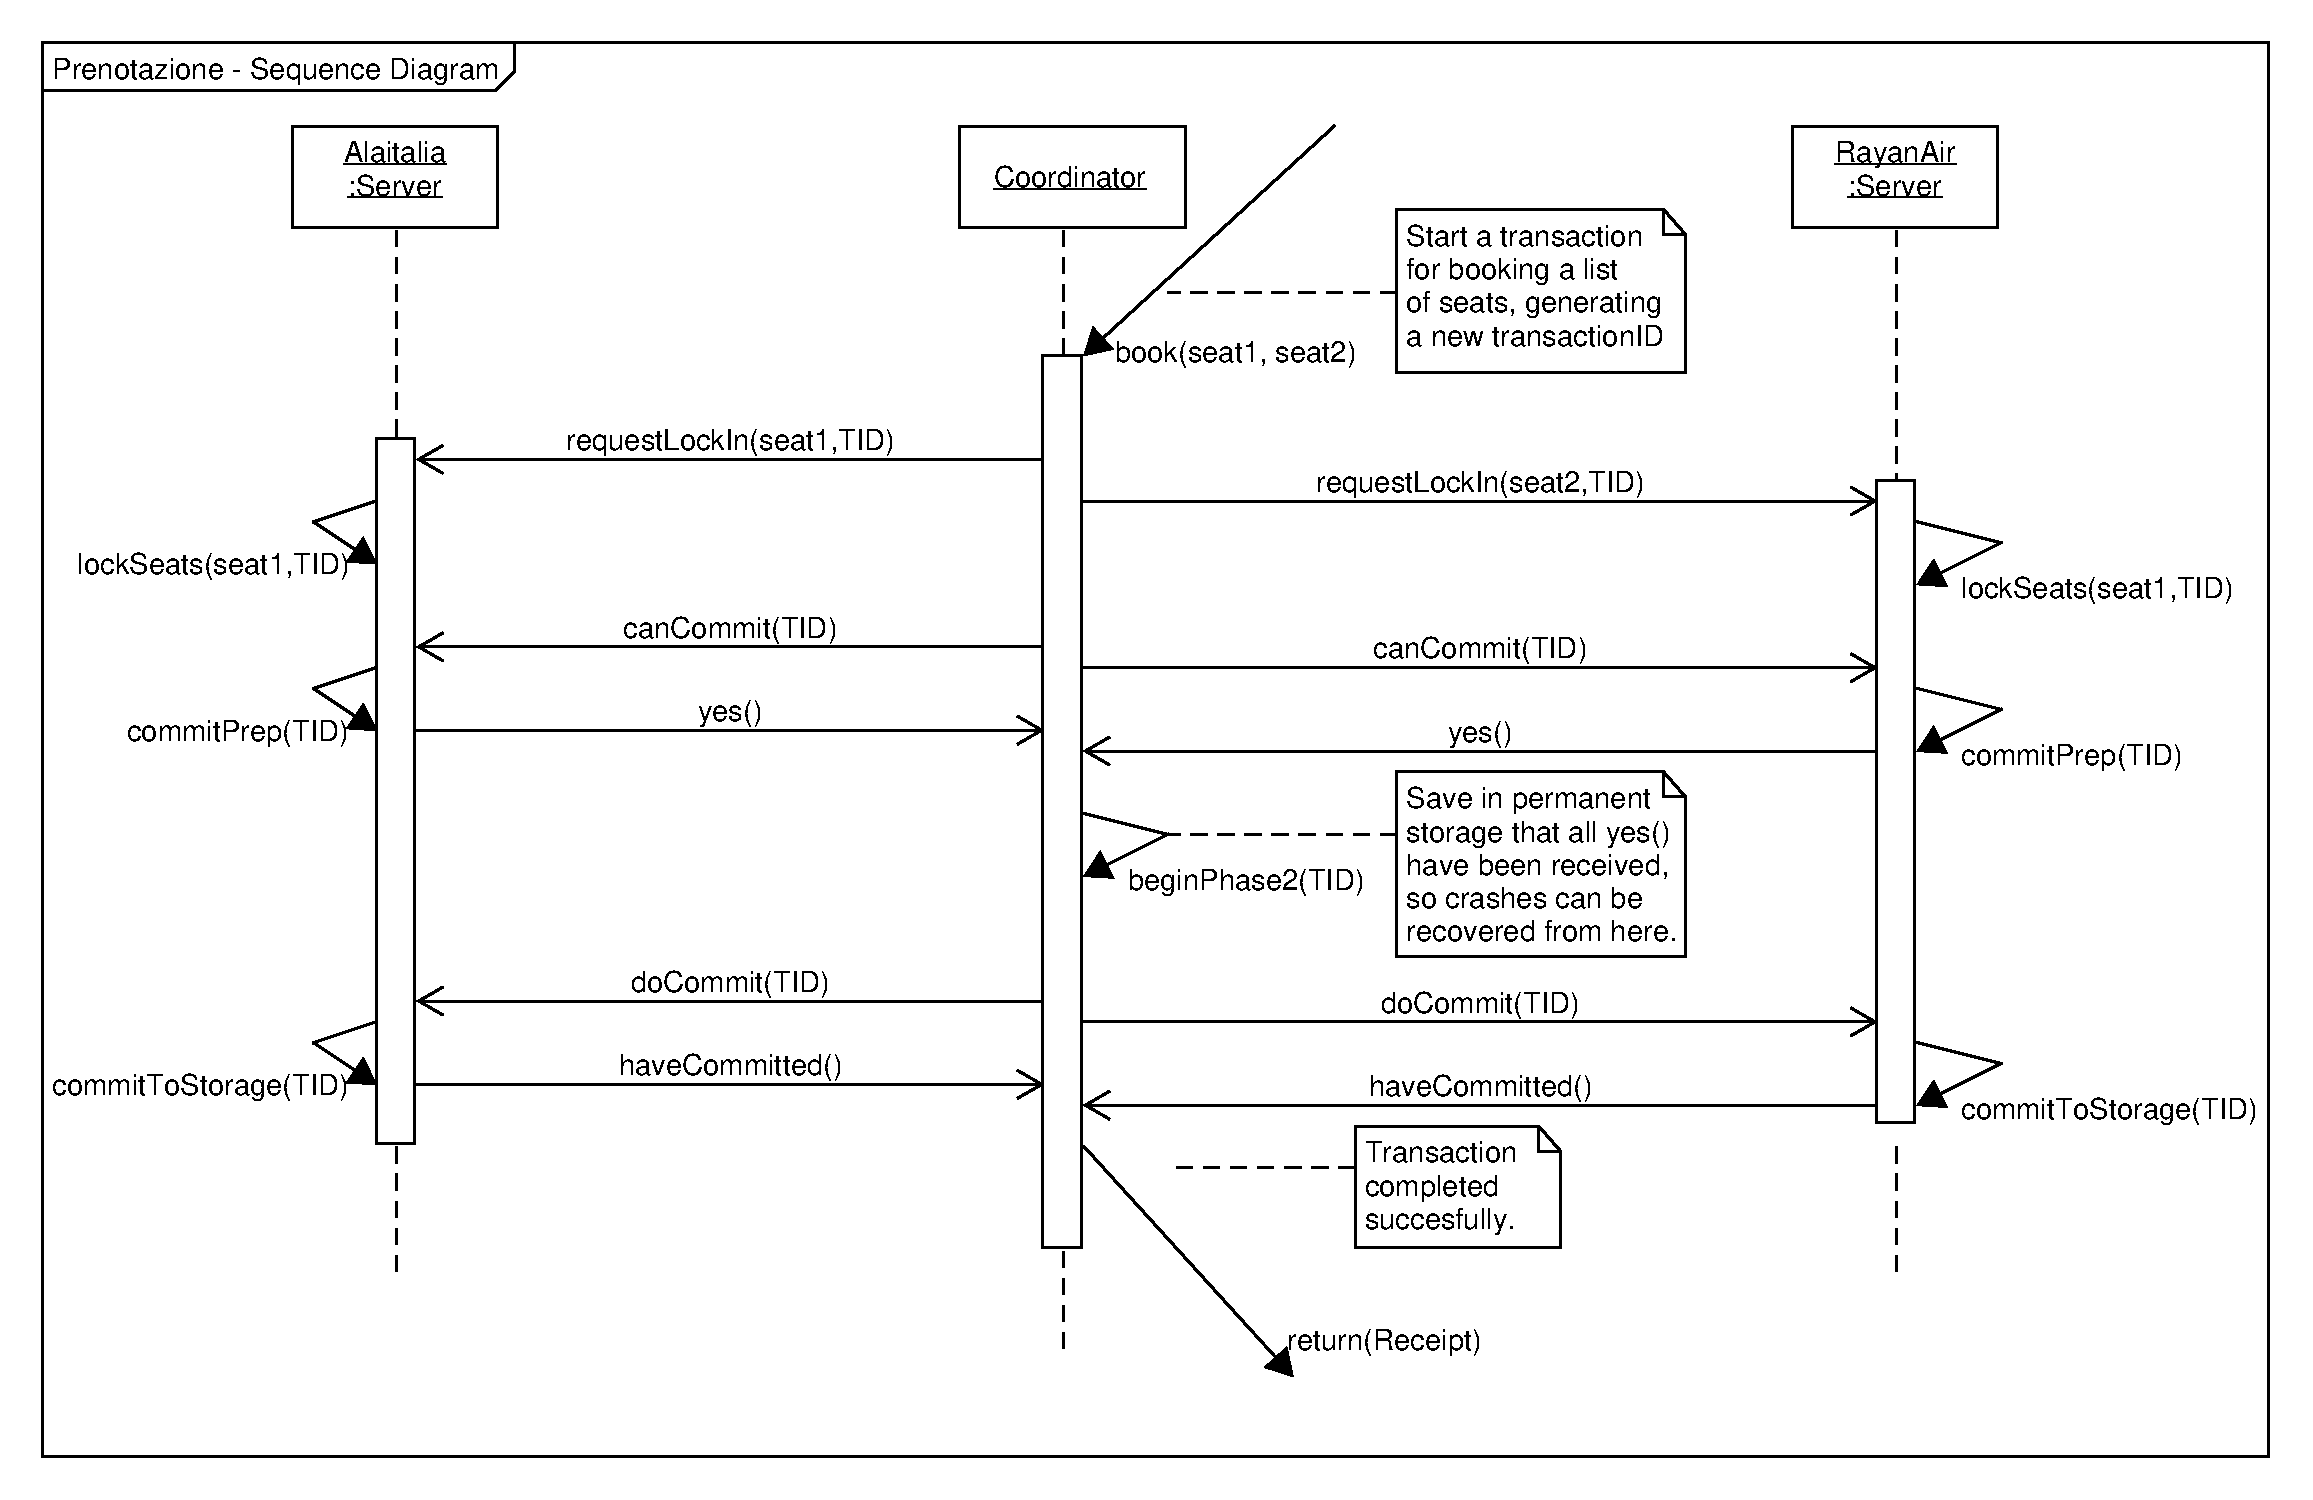
\includegraphics[width=\textwidth]{fig/reserve_sequence.pdf}
		\caption{Diagramma di sequenza UML di un'operazione di prenotazione di due posti, eseguita con successo.}
		\label{fig:bookseq}
\end{figure}

\paragraph{Lista posti}La richiesta della lista di posti disponibili � una semplice interrogazione di tipo \textit{request-reply}: il server invia la lista di tutti i voli e relativi posti, compreso il loro stato (disponibile/occupato).

\paragraph{Prenotazione}Come mostrato in figura \ref{fig:bookseq}, l'operazione di prenotazione consiste nel richiedere il \textit{lock} delle risorse ai server coinvolti, per poi inizializzare un \textit{two phase commit protocol}.
Se le risorse non sono disponibili, allora il protocollo 2PC far� abortire la transazione.


Il ruolo di coordinatore della transazione pu� essere assunto sia dal client che da un server (work in progress). 

Tutte le parti coinvolte sfruttano dei file di \textit{log} per eseguire il recupero dai guasti.

%============================================================================

\subsection{Architettura fisica}
% Nodi e piattaforme coinvolte, dove vengono piazzati


%============================================================================
%============================================================================
%============================================================================

\end{document}














